\begin{wrapfigure}[0]{r}[-1.5cm]{3cm}
 \vspace{-6cm}
 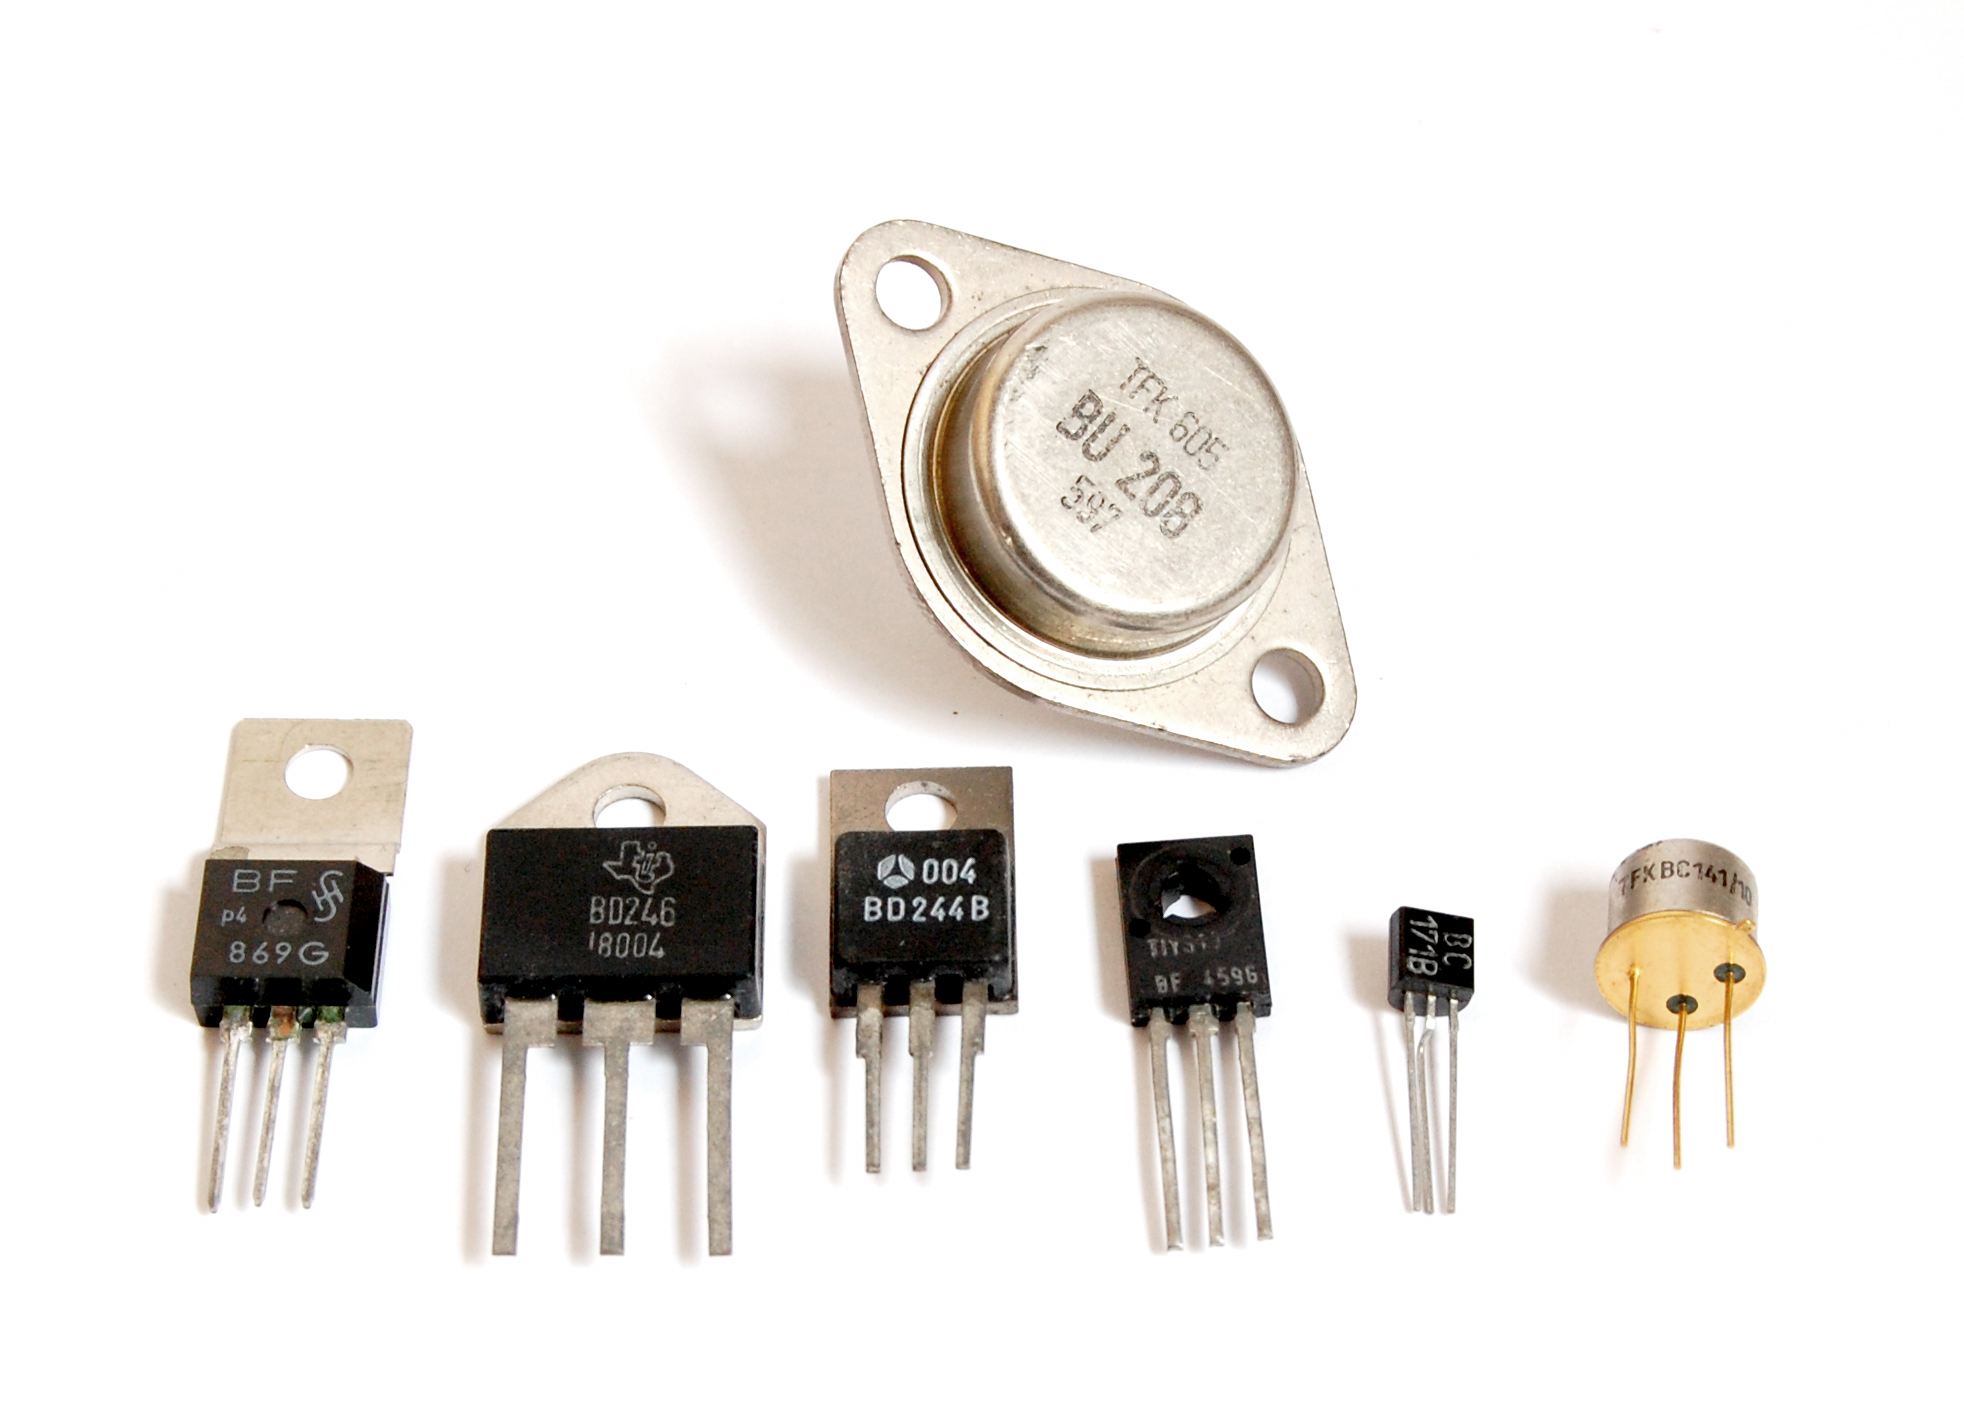
\includegraphics[scale=0.3]{Transistor/Bilder/Transistors-white.jpg}
 \vspace{-6cm}
\end{wrapfigure}

\section*{Theorie- und Prüfungsfragen} 


\mucho{1}{TC607}
{Welche Kollektorspannungen haben NPN- und PNP-Transistoren?}%Frage
{NPN-Transistoren benötigen positive, PNP-Transistoren negative Kollektorspannungen.}%A
{NPN- und PNP-Transistoren benötigen negative Kollektorspannungen.}%B
{PNP-Transistoren benötigen positive, NPN-Transistoren negative Kollektorspannung.}%C
{PNP- und NPN-Transistoren benötigen positive Kollektorspannungen.}%D
{A}%Lösung

\mucho{2}{TC612}
{Wie groß ist die Basisspannung eines NPN-Silizium-Transistors, wenn sich dieser in leitendem Zustand befindet?}%Frage
{Sie ist viel höher als die Emitterspannung.}%A
{Sie entspricht der Kollektorspannung.}%B
{Sie ist etwa 0,6 V höher als die Emitterspannung.}%C
{Sie liegt etwa 0,6V unter der Emitterspannung.}%D
{C}%Lösung

\aufgabentext{
	\begin{enumerate}
	\item[3] Wie werden die Mosfets in der folgenden Abbildung richtig bezeichnet?
	\end{enumerate}
	A 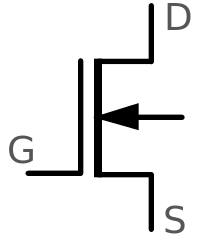
\includegraphics[scale=0.2]{Transistor/Bilder/MOSFET-Symbole1.png}
	B 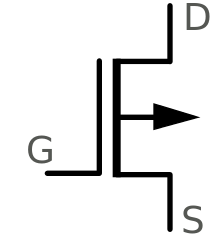
\includegraphics[scale=0.2]{Transistor/Bilder/MOSFET-Symbole2.png}
	C 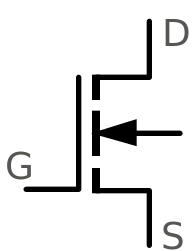
\includegraphics[scale=0.2]{Transistor/Bilder/MOSFET-Symbole3.png}
	D 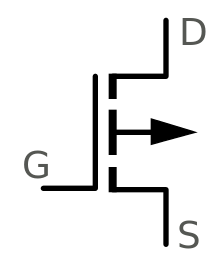
\includegraphics[scale=0.2]{Transistor/Bilder/MOSFET-Symbole4.png}
	\loesung{Lösung: A selbstleitender n-Kanal Mosfet, B selbstleitender p-Kanal Mosfet, C selbstsperrender n-Kanal Mosfet, D selbstsperrender p-Kanal Mosfet}
	}


\aufgabentext{
	\begin{enumerate}
	\item[4] \textbf{TD431} Das folgende Signal wird an den Eingang nebenstehender Schaltung gelegt. Welches ist ein mögliches Ausgangssignal U2?\\
	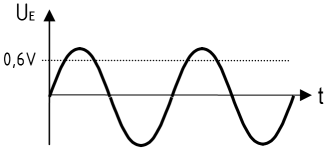
\includegraphics[scale=0.4]{Transistor/Bilder/TD431_0.png}
	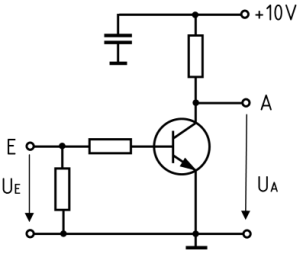
\includegraphics[scale=0.35]{Transistor/Bilder/TD4x2.png}
	\end{enumerate}
	A 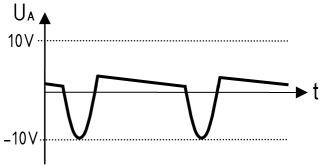
\includegraphics[scale=0.3]{Transistor/Bilder/TD431_A.png}
	B 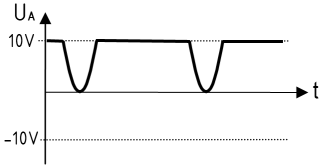
\includegraphics[scale=0.3]{Transistor/Bilder/TD431_B.png}\\
	C 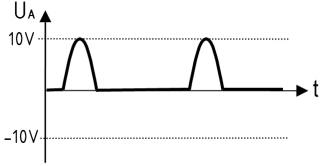
\includegraphics[scale=0.3]{Transistor/Bilder/TD431_C.png}
	D 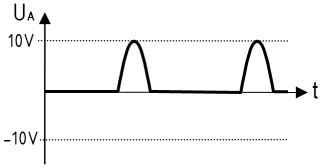
\includegraphics[scale=0.3]{Transistor/Bilder/TD431_D.png}
	\loesung{Lösung: B}
	}

\vspace*{0.65cm}

\mucho{5}{TC618}
{Die Betriebsspannung beträgt 10 V, der Kollektorstrom soll 2 mA betragen, die Gleichstromverstärkung des Transistors beträgt 200. Berechnen Sie den Vorwiderstand R1.\\
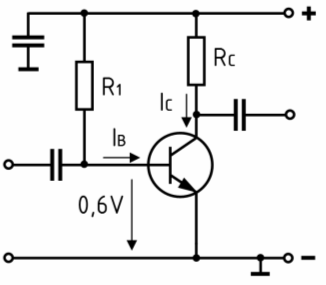
\includegraphics[scale=0.4]{Transistor/Bilder/TC618.png}
}%Frage
{1$M\Omega$}%A
{940$K\Omega$}%B
{85,5$K\Omega$}%C
{47$K\Omega$}%D
{B \hspace{3em} mit $B = \frac{I_C}{I_B}$ und $I_C = 2mA$ sowie $B = 200$ \\
    $$\rightarrow I_C = 200 \cdot I_B \rightarrow R 
    = \frac{U}{I} = \frac{10V - 0,6 V}{\frac{2 mA}{200}}$$}%Lösung

\mucho{6}{TD401 }
{Bei dieser Schaltung handelt es sich um\\
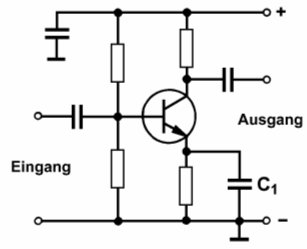
\includegraphics[scale=0.4]{Transistor/Bilder/TD403.png}
}%Frage
{einen Verstärker in Kollektorschaltung.}%A
{einen Verstärker in Basisschaltung.}%B
{einen Verstärker in Emitterschaltung.}%C
{einen Verstärker als Emitterfolger.}%D
{C}%Lösung

\mucho{7}{TD403 }
{Welche Funktion hat der Kondensator C1 in der  Schaltung in Aufgabe 6?\\
}%Frage
{Verringerung der Verstärkung.}%A
{Überbrückung des Emitterwiderstandes für das Wechselstromsignal.}%B
{Stabilisierung des Arbeitspunktes des Transistors.}%C
{Einstellung der Vorspannung am Emitter.}%D
{B}%Lösung

\mucho{8}{TD406 }
{Was lässt sich über die Wechselspannungsverstärkung $v_U$ und die Phasenverschiebung $\phi$ zwischen Ausgangs- und Eingangsspannung der Schaltung in Aufgabe 6 aussagen?\\
}%Frage
{$v_U$ ist groß (z.B. 100 ... 300) und $\phi=180^\circ$.}%A
{$v_U$ ist groß (z.B. 100 ... 300) und $\phi=0^\circ$.}%B
{$v_U$ ist klein (z.B. 0,9 ... 0,98) und $\phi=180^\circ$.}%C
{$v_U$ ist klein (z.B. 0,9 ... 0,98) und $\phi=0^\circ$.}%D
{A}%Lösung
